%package list
\documentclass{article}
\usepackage[top=3cm, bottom=3cm, outer=3cm, inner=3cm]{geometry}
\usepackage{graphicx}
\usepackage{url}
%\usepackage{cite}
\usepackage{hyperref}
\usepackage{array}
%\usepackage{multicol}
\newcolumntype{x}[1]{>{\centering\arraybackslash\hspace{0pt}}p{#1}}
\usepackage{natbib}
\usepackage{pdfpages}
\usepackage{multirow}
\usepackage{multirow}
\usepackage[normalem]{ulem}
\useunder{\uline}{\ul}{}



%%%%%%%%%%%%%%%%%%%%%%%%%%%%%%%%%%%%%%%%%%%%%%%%%%%%%%%%%%%%%%%%%%%%%%%%%%%%
%%%%%%%%%%%%%%%%%%%%%%%%%%%%%%%%%%%%%%%%%%%%%%%%%%%%%%%%%%%%%%%%%%%%%%%%%%%%
\newcommand{\csemail}{vmachacaa@ulasalle.edu.pe}
\newcommand{\csdocente}{MSc. Vicente Enrique Machaca Arceda}
\newcommand{\cscurso}{Fundamentos de Lenguajes de
Programación}
\newcommand{\csuniversidad}{Universidad La Salle}
\newcommand{\csescuela}{Escuela Profesional de Ingeniería de Software}
\newcommand{\cspracnr}{04}
\newcommand{\cstema}{Ensamblador}
%%%%%%%%%%%%%%%%%%%%%%%%%%%%%%%%%%%%%%%%%%%%%%%%%%%%%%%%%%%%%%%%%%%%%%%%%%%%
%%%%%%%%%%%%%%%%%%%%%%%%%%%%%%%%%%%%%%%%%%%%%%%%%%%%%%%%%%%%%%%%%%%%%%%%%%%%


\usepackage[english,spanish]{babel}
\usepackage[utf8]{inputenc}
\AtBeginDocument{\selectlanguage{spanish}}
\renewcommand{\figurename}{Figura}
\renewcommand{\refname}{Referencias}
\renewcommand{\tablename}{Tabla} %esto no funciona cuando se usa babel
\AtBeginDocument{%
	\renewcommand\tablename{Tabla}
}

\usepackage{fancyhdr}
\pagestyle{fancy}
\fancyhf{}
\setlength{\headheight}{30pt}
\renewcommand{\headrulewidth}{1pt}
\renewcommand{\footrulewidth}{1pt}
\fancyhead[L]{\raisebox{-0.2\height}{
\includegraphics[width=3cm]{img/logo_salle}}}
\fancyhead[C]{}
\fancyhead[R]{\fontsize{7}{7}\selectfont	\csuniversidad \\ \csescuela \\ \textbf{\cscurso} }
\fancyfoot[L]{MSc. Vicente Machaca}
\fancyfoot[C]{\cscurso}
\fancyfoot[R]{Página \thepage}

\usepackage{listings}
\usepackage{xcolor} % for setting colors

% set the default code style
\lstset{
    frame=tb, % draw a frame at the top and bottom of the code block
    tabsize=4, % tab space width
    showstringspaces=false, % don't mark spaces in strings
    numbers=left, % display line numbers on the left
    commentstyle=\color{green}, % comment color
    keywordstyle=\color{blue}, % keyword color
    stringstyle=\color{red} % string color
}






\begin{document}
	\nocite{10.5555/1610485}
	\vspace*{10px}
	
	\begin{center}	
		\fontsize{17}{17} \textbf{ Práctica \cspracnr}
	\end{center}
	%\centerline{\textbf{\underline{\Large Título: Informe de revisión del estado del arte}}}
	%\vspace*{0.5cm}
	

	\begin{table}[h]
		\begin{tabular}{|x{4.7cm}|x{4.8cm}|x{4.8cm}|}
			\hline 
			\textbf{DOCENTE} & \textbf{CARRERA}  & \textbf{CURSO}   \\
			\hline 
			\csdocente & \csescuela & \cscurso    \\
			\hline 
		\end{tabular}
	\end{table}	
	
	
	\begin{table}[h]
		\begin{tabular}{|x{4.7cm}|x{4.8cm}|x{4.8cm}|}
			\hline 
			\textbf{PRÁCTICA} & \textbf{TEMA}  & \textbf{DURACIÓN}   \\
			\hline 
			\cspracnr & \cstema & 3 horas   \\
			\hline 
		\end{tabular}
	\end{table}
	
	
	\section{Datos de los estudiantes}
	\begin{itemize}
		\item GIT: \href{https://github.com/Robertohg/FLP}{GIT-Repo}
		\item Integrantes: 
		\begin{itemize}
			\item Roberto Heredia Garland
			
		\end{itemize}		
	\end{itemize}
	
	
	

	
	\section{Ejercicios}\label{sec:ejercicios}
	\begin{enumerate}
		\item Cree un array de 5 elementos con múltiplos de un número ingresado por teclado, luego debe mostrar dicho array por pantalla.
	

	
		\begin{lstlisting}[language={[x86masm]Assembler}, basicstyle=\small]

..data
	txt1: .asciiz "Ingrese un numero: "
	txt2: .asciiz "Los multiplos de "
	txt3: .asciiz " son:"
	arr: .word	1, 2, 3, 4, 5
	txt4: .asciiz "\n"
.text
main:
	li $v0,4
	la $a0, txt1
	syscall

	li $v0,5 
	syscall

	move $t3, $v0 
	
	
	li $v0,4
	la $a0, txt2
	syscall

	move $a0, $t3

	li $v0,1
	syscall

	li $v0,4
	la $a0, txt3
	syscall

	li $t0, 0 
    	la $t1, arr

	loop1:
    		bge     $t0, 5, exit
    
    		lw      $t2, 0($t1)
    		add    $t1, $t1, 4

		mul $t6, $t2, $t3 
		li $v0,4
		la $a0, txt4
		syscall

    		li      $v0, 1    
    		move    $a0, $t6 
    		syscall
		
		li      $a0, 32 
    		li      $v0, 11  
    		syscall
    
    		add    $t0, $t0, 1 
    		j      loop1
	exit:

	jr $ra

	
		   \end{lstlisting}
	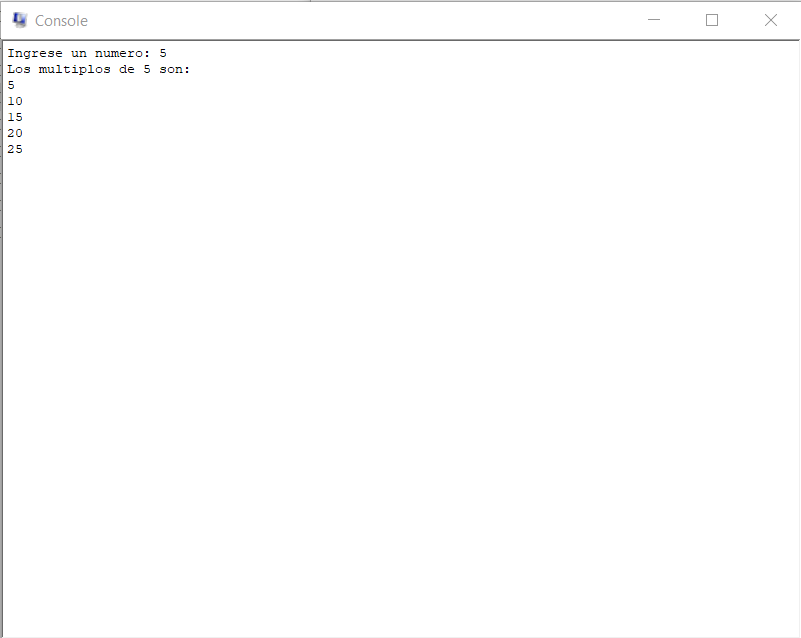
\includegraphics[width=8cm]{img/eje1.png}
	\newpage
	\item Cree un programa que solicite 5 elementos por teclado y los almacene en un Array. Luego se debe mostrar estos elementos en orden inverso.
	
		\begin{lstlisting}[language={[x86masm]Assembler}, basicstyle=\small]
.data 
    	txt1: .asciiz "Ingrese un numero: "
    	txt2: .asciiz "Elementos inversos:\n"
	arr: .word	1:5 
    
.text 
main: 
	li $t0, 0
    	li $t2, 0
    	la $t1, arr
loop1:
    	bge $t0, 5, end_loop1
    
    	li $v0, 4
    	la $a0, txt1
    	syscall
    
    	li  $v0,5 
    	syscall
    	move $t2, $v0
    
    	sw $t2, 0($t1) 
    	add $t1, $t1, 4 
    	add $t0, $t0, 1 
    	j loop1

end_loop1:

    	sub $t1, $t1,4
    	li $t0, 0
    	
    	li $v0, 4
    	la $a0, txt2
    	syscall

loop2:
    	bge $t0, 5, end_loop2
    	lw $t2, 0($t1)
    	sub $t1, $t1, 4

    	li $v0, 1      
    	move $a0, $t2
    	syscall

    	li $a0, 32

    	li $v0, 11
    	syscall
    	add $t0, $t0, 1	#i++

    	j loop2

end_loop2:

    	jr $ra
		   \end{lstlisting}	
	
	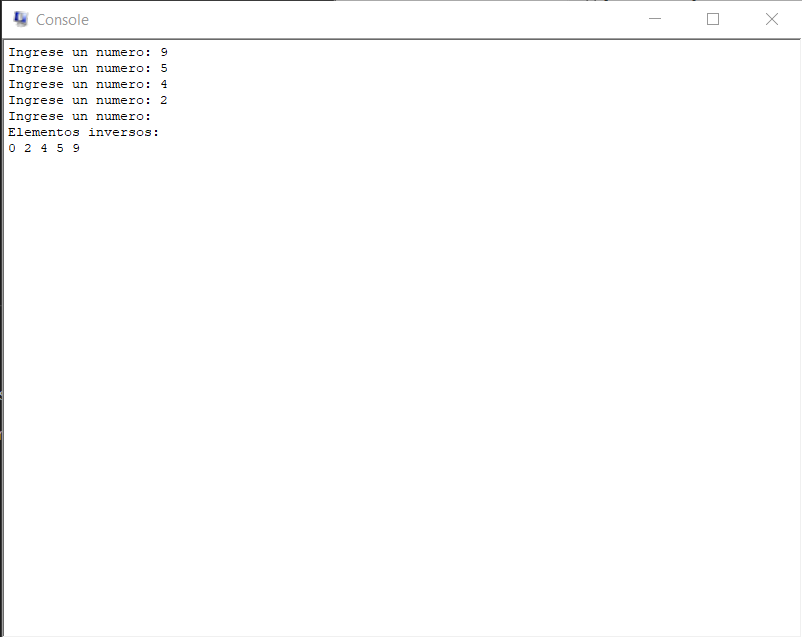
\includegraphics[width=8cm]{img/eje2.png}
	
	\clearpage
	%\bibliographystyle{apalike}
	%\bibliographystyle{IEEEtranN}
	%\bibliography{bibliography}
		\end{enumerate}
	
\end{document}